\chapter{研究の準備}\label{cha:Preparation}
  \vspace{-2zh}
本章では、本研究で必要となる前提知識を説明する。
% \section{モータ作成}\label{motor}
% \subsection{仕様書}\label{siyo}
% \subsection{シミュレータの役割}\label{simu}
  \vspace{-1zh}
\section{Modelica言語}\label{modelica}
Modelica言語とは、微分代数方程式を用いた、複合領域のマルチドメインモデリングのために開発されたオブジェクト指向言語である\cite{modelicaモデルベース本}。
Modelica言語仕様は、非営利団体のModelica Associationが策定している。
Modelica Associationでは、Modelica言語による様々な物理領域のモデルライブラリを開発しており、
数学、機械、電気、熱、流体、制御系、状態遷移機械などを含んだフリーウェアのModelica標準ライブラリ(Modelica Standard Library : MSL)をリリースしている
\cite{modelicaモデルベース本}。
  \vspace{-1zh}
\section{OpenModelica}\label{OM}
OpenModelicaとは、Open Source Modelica Consortium (OSMC)が開発しているModelicaコードのモデリング、シミュレーション、デバッグのための機能などを
持つオープンソースプラットフォームである\cite{fritzson2006openmodelica}。
OpenModelicaでは、グラフィカルにモデリングすることが可能であり、専用のグラフィカルモデルエディタが用意されている。グラフィカルモデルエディタの外観を、図\ref{fig:OM_GUI}に示す。
また、グラフィカルモデルエディタ上にモデルを配置する際、オブジェクト名の確認をポップアップウィンドウで行う。ポップアップウィンドウの例を、図\ref{fig:name_ob}に示す。
\begin{figure}[t]
	\centering
	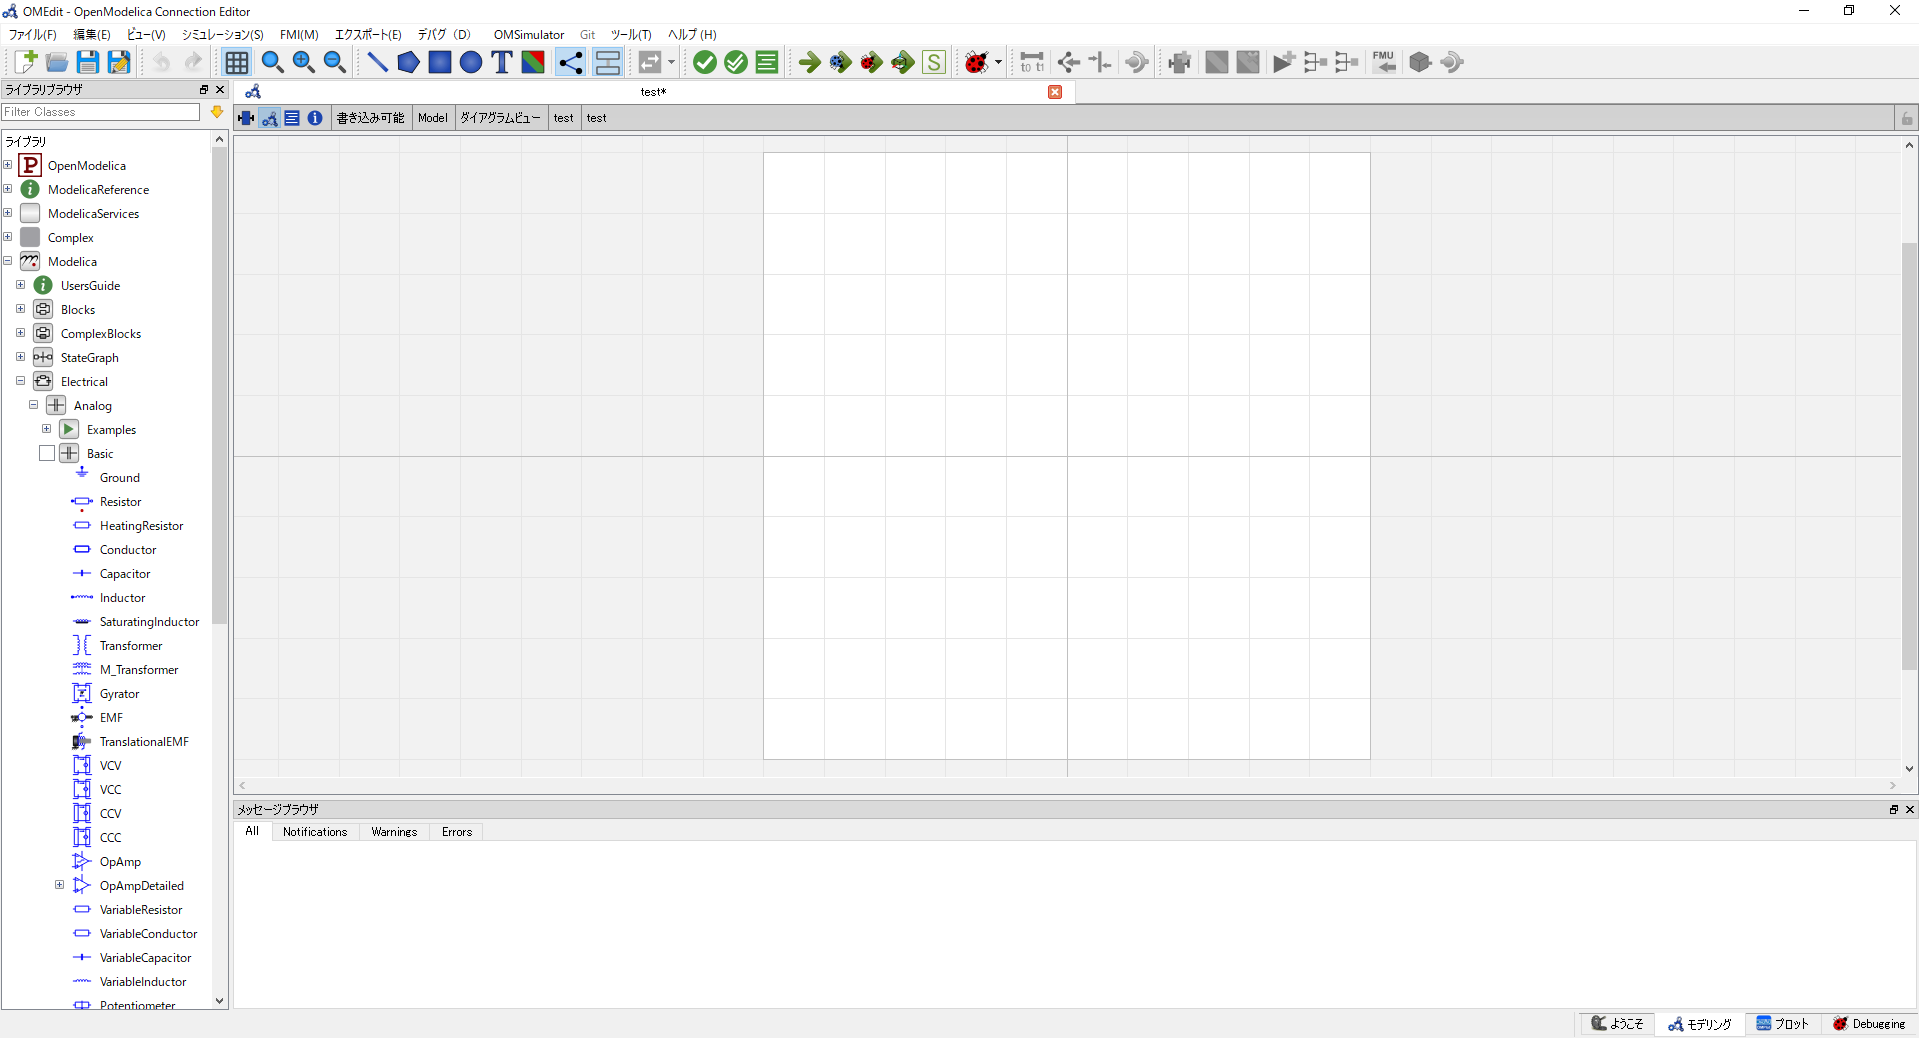
\includegraphics[width=16.5cm,height=10cm]{./Image/OM_GUI.png}
	\caption{グラフィカルモデルエディタの外観}
	\label{fig:OM_GUI}
\end{figure}
\begin{figure}[t]
	\centering
	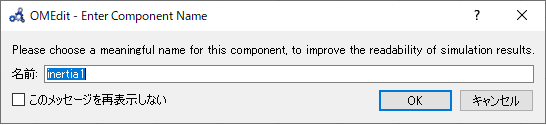
\includegraphics[width=12cm]{./Image/name_ob.png}
	\caption{オブジェクト名を確認するポップアップウィンドウの例}
	\label{fig:name_ob}
\end{figure}
% 本論文では、OpenModelica上でグラフィカルにモデリングしたモデルを「Modelicaモデル」、Modelicaモデルのソースコードを「Modelicaコード」と呼称する。
OpenModelicaは、シミュレーション結果をグラフとして画面上に描画できる。また、シミュレーション結果は、以下の3つのファイル形式で保存できる。
\begin{itemize}
    \item matファイル
    \item pltファイル
    \item csvファイル
\end{itemize}

今回試作するモータ特性表自動生成ツールでは、csvファイルにのみ対応する。

OpenModelicaから出力されるcsvファイルの一部を、図\ref{fig:simyu_csv}に示す。

OpenModelicaから出力されるcsvファイルの1行目の各列には、オブジェクト名が入る。
1列目には、シミュレーションにおける経過時間を示すデータを格納し、2列目以降には、シミュレーションにおける経過時間ごとの各オブジェクトの値を格納する。
% 図\ref{fig:simyu_csv}に示すcsvファイルの1列目には、「0.0秒」から始まる時刻を表すデータが必ず入る。
% そして1行目には、1列目の「time」を除いて、オブジェクト名を含んだ変数名が必ず入る。また以降には、1列目の「time」における各変数の値が2列目以降にそれぞれ入る。
% また、2行目には、時刻が「0.0秒」の時の各変数の値が必ず入る。

OpenModelicaから出力されるcsvファイルのファイル名は、「(シミュレーションしたモデルの名前)\_res.csv」で生成される。
例えば、シミュレーションに用いたモデルの名前が「hoge」だった場合、csvファイルのファイル名は「hoge\_res.csv」となる。
\begin{figure}[t]
	\centering
	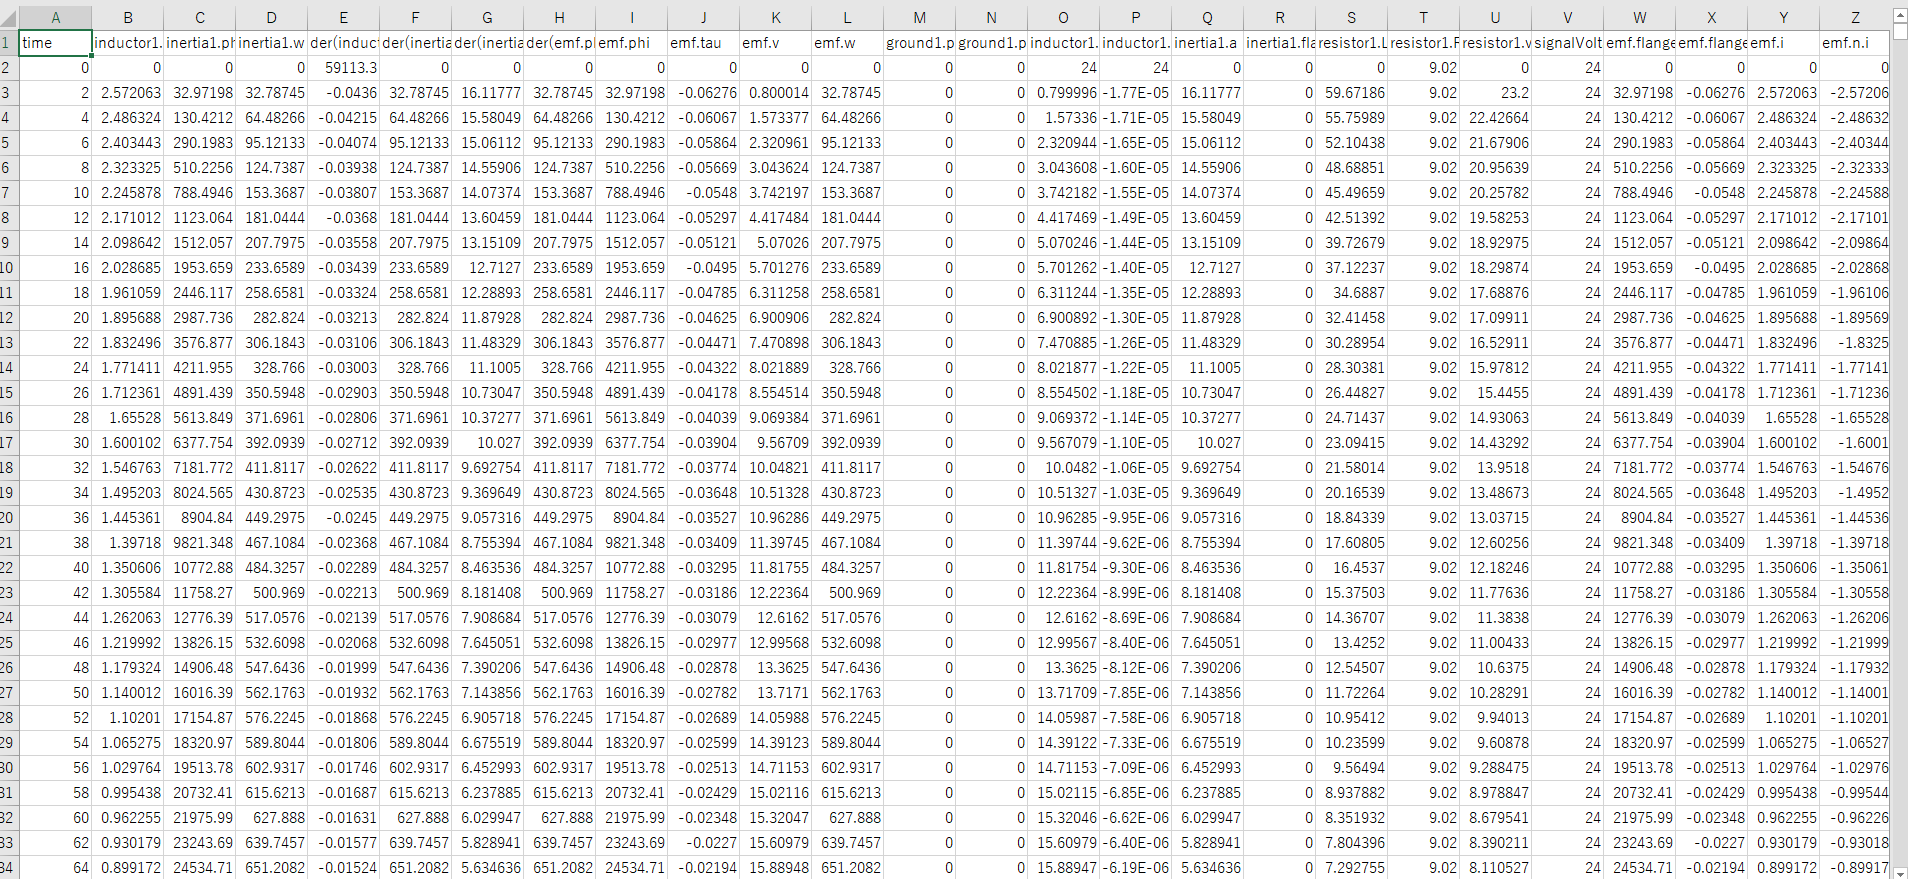
\includegraphics[width=16.5cm,height=10cm]{./Image/simyu_csv.png}
	\caption{シミュレーション結果であるcsvファイルの一部}
	\label{fig:simyu_csv}
\end{figure}
% 試作するモータ特性表自動生成ツールでは、OpenModelica 1.9.1 Beta1を使用する。
\section{ブラシ付きDCモータ}\label{bDCmotor}
% ブラシ付きDCモータだけかけばいいのか?モータ全体の話も必要か?
DCモータとは、磁場の中にあるコイルに電流を流す事で発生するローレンツ力を回転方向に利用することで回すモータである\cite{モータ原理}。
また、ブラシ付きDCモータとは、モータ内部に「ブラシ」と呼ばれる電極と、「コミュテータ」と呼ばれる整流子を設け、その二つを接触させ機械的に電流の切り替えを行うことによって回す、DCモータである。
ブラシ付きDCモータは、シンプルな構造で、制御が容易で汎用性が高く、模型用モータや自動車補機用モータなど、世界で一番多く使われているモータである\cite{モータ使う}。
% 3章へ
%   今回試作するモータ特性表自動生成ツールでは、ブラシ付きモータのシミュレーション結果にのみ対応する。
\section{対象とするモデル}\label{taioumodel}
試作するモータ特性表自動生成ツールでは、以下に示す2つのModelicaモデルのシミュレーション結果を対象とする。
\begin{itemize}
	\item ブラシ付きDCモータのModelicaモデル
	\item ブラシ付きDCモータのModelicaモデルをサブシステムとするモデル
\end{itemize}

以下で、それぞれ説明する。
% \begin{itemize}
% 	\item ブラシ付きDCモータのModelicaモデル
% 	\item ブラシ付きDCモータのModelicaモデルをサブシステムとするモデル
% \end{itemize}
% 以下に上記のモデルについて具体的に説明する。
\subsection{ブラシ付きDCモータのModelicaモデル}\label{sub:tanntai}
ブラシ付きDCモータのModelicaモデルとは、ブラシ付きDCモータの等価回路\cite{等価回路}をModelica言語で表したモデルのことである。
ブラシ付きDCモータの等価回路を、図\ref{fig:touka}に示す。また、ブラシ付きDCモータのModelicaモデルの例を図\ref{fig:tantai_model}に示す。
\begin{figure}[t]
	\centering
	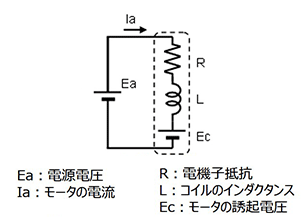
\includegraphics[width=7cm]{./Image/touka.png}
	\caption{ブラシ付きDCモータの等価回路}
	\label{fig:touka}
  \end{figure}
ブラシ付きDCモータの等価回路をModelica言語で表すためには、電源部品、抵抗部品、インダクタ部品、起電力部品、慣性部品、接地部品が必要である。
% 上記6つの部品が必要な理由は、ブラシ付きDCモータの等価回路\cite{等価回路}をModelica言語で表す際に、使用する部品\cite{modelicaシステム本}だからである。\\

また、電源部品、抵抗部品、インダクタ部品、起電力部品、慣性部品には、それぞれ以下のパラメータを設定しなければならない。
各部品で使用するMSLを、表\ref{tab:MSL}に示す。
\begin{itemize}
	\item 電源部品 ・・・ 電圧値 $(\mathrm{V})$
	\item 抵抗部品 ・・・ 抵抗値 ($\Omega$)
	\item インダクタ部品 ・・・ インダクタンス値 $(\mathrm{H})$
	\item 起電力部品 ・・・ トルク定数 ($\mathrm{N\cdot m/A}$)
	\item 慣性部品 ・・・ 慣性モーメント ($\mathrm{kg\cdot m^2}$)
\end{itemize}

% 図\ref{fig:tantai_model}が持つ変数の一覧を図\ref{fig:hensuu}に、
%図\ref{fig:tantai_model}のModelicaコードを図\ref{fig:tantai_modelica}に、
% 図\ref{fig:hensuu}は、
\begin{figure}[t]
	\centering
	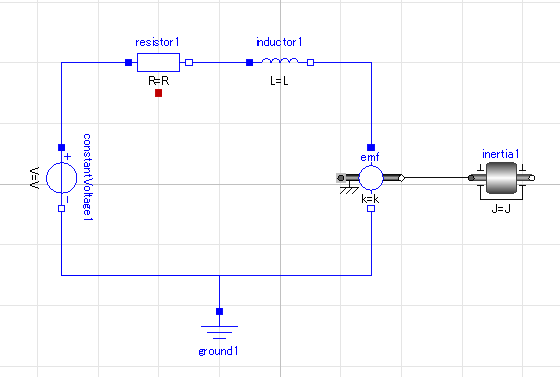
\includegraphics[width=10cm]{./Image/tantai_model.png}
	\caption{ブラシ付きDCモータのModelicaモデルの例}
	\label{fig:tantai_model}
  \end{figure}
  

\begin{table}[t]
	\centering
	\caption{MSL対応表}
	\begin{tabular}{|c|c|} \hline
	  部品名 & 使用するMSL \\ \hline \hline
	  電源部品 & Modelica.Electrical.Analog.Sources \\ \hline
	  抵抗部品 & Modelica.Electrical.Analog.Basic \\ \hline
	  インダクタ部品 & Modelica.Electrical.Analog.Basic \\ \hline
	  起電力部品 & Modelica.Electrical.Analog.Basic \\ \hline
	  慣性部品 & Modelica.Mechanics.Rotational.Components \\ \hline
	  接地部品 & Modelica.Electrical.Analog.Basic \\ \hline
	\end{tabular}
	\label{tab:MSL}
  \end{table}


% \begin{figure}[t]
% 	\centering
% 	\fbox{
% 	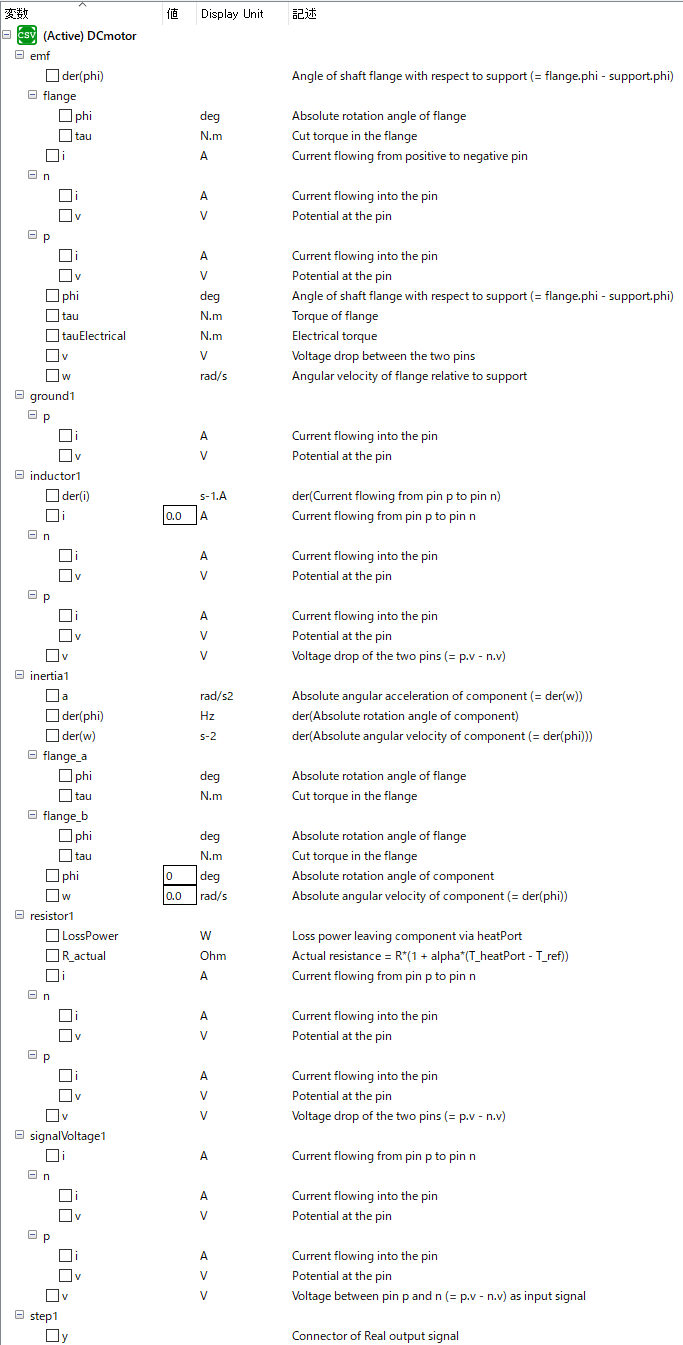
\includegraphics[width=11.5cm]{./Image/part.png}
% 	}
% 	\caption{図\ref{fig:tantai_model}が持つ変数の一覧}
% 	\label{fig:hensuu}
%   \end{figure}
  
\clearpage
% \begin{figure*}[t]
% 	\lstinputlisting[label={code:motor}, caption={図\ref{fig:tantai_model}のModelicaコード}]{./chapters/motor.mo}
% \end{figure*}

% \begin{figure}[t]
% 	\centering
% 	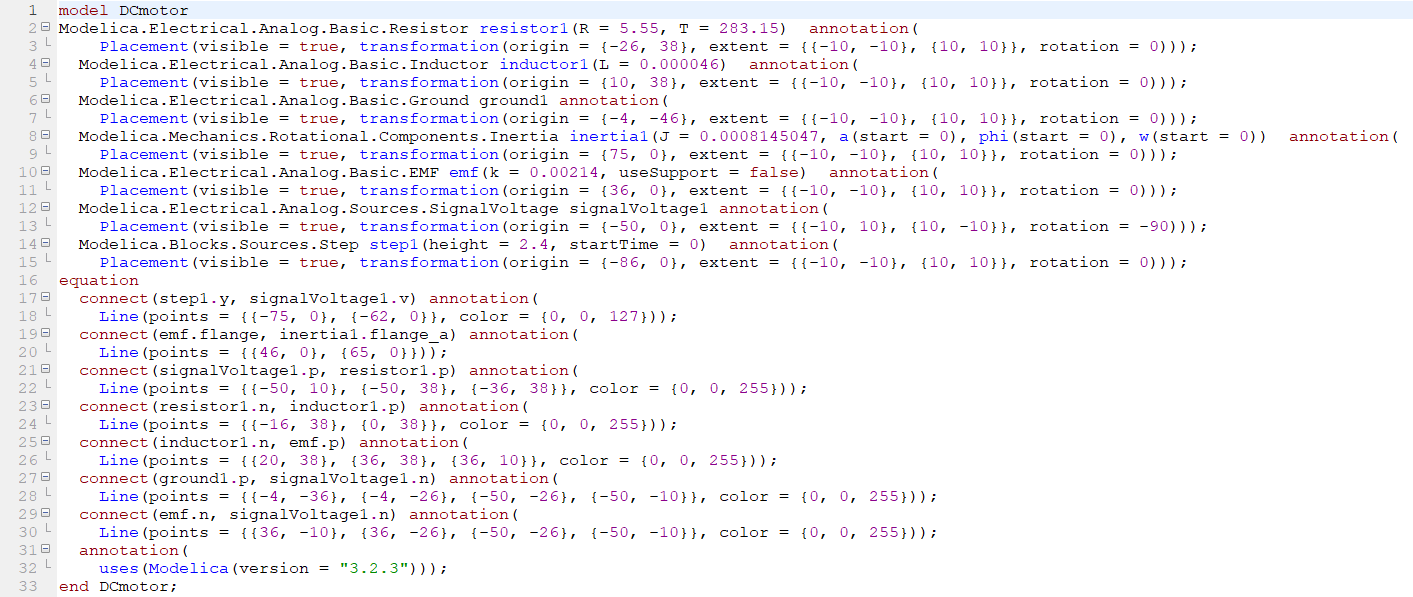
\includegraphics[width=16.5cm,height=8cm]{./Image/tantai_modelica.png}
% 	\caption{図\ref{fig:tantai_model}のModelicaコード}
% 	\label{fig:tantai_modelica}
%   \end{figure}

%   \vspace{-1zh}

\subsection{ブラシ付きDCモータのModelicaモデルをサブシステムとするモデル} \label{sub:submodel}
ブラシ付きDCモータのModelicaモデルをサブシステムとするモデルとは、
\ref{sub:tanntai}節で説明したブラシ付きDCモータのModelicaモデルを1つのサブシステムとして扱い、他の部品と組み合わせ作成したモデルのことである。

例として、ブラシ付きDCモータのサブシステムを用いたDCサーボモータのモデルを、図\ref{fig:submodel}に
%図\ref{fig:submodel}のModelicaコードを図\ref{fig:sub_modelica}に、
示す。

\begin{figure}[t]
	\centering
	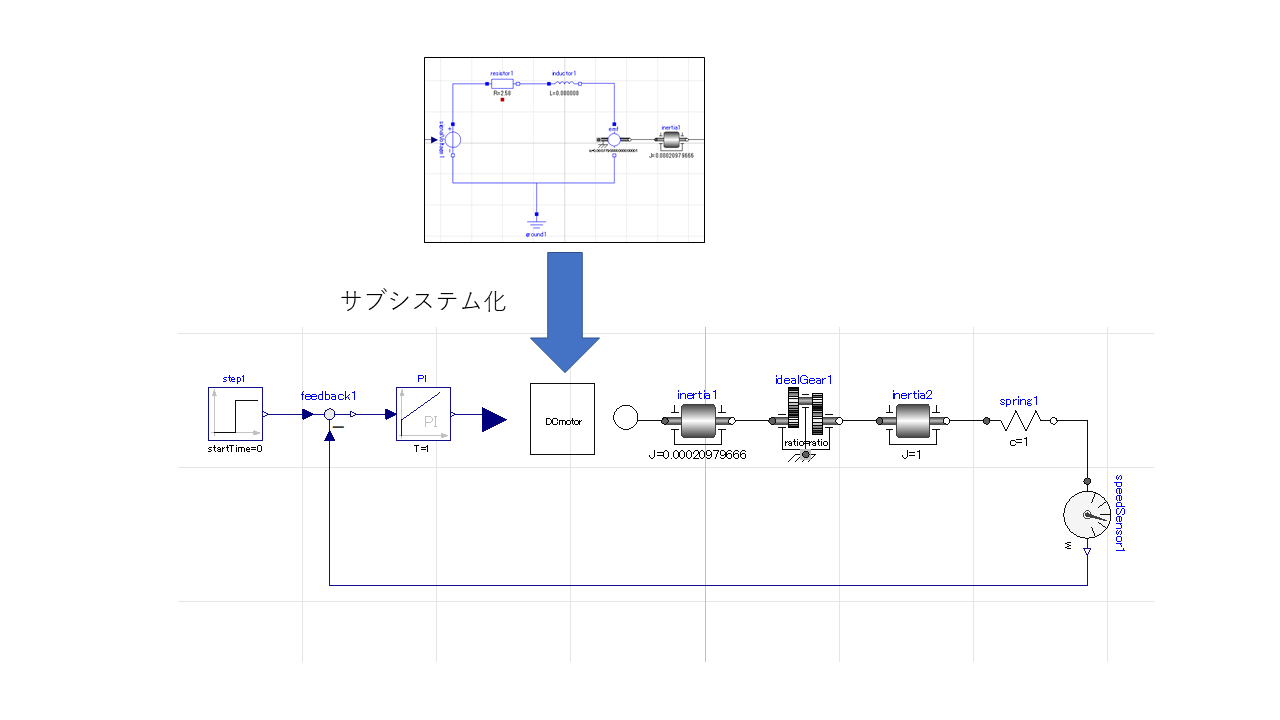
\includegraphics[width=16.5cm,height=10cm]{./Image/submodel_pack.png}
	\caption{DCサーボモータのモデル}
	\label{fig:submodel}
  \end{figure}

%   \begin{figure}[t]
% 	\centering
% 	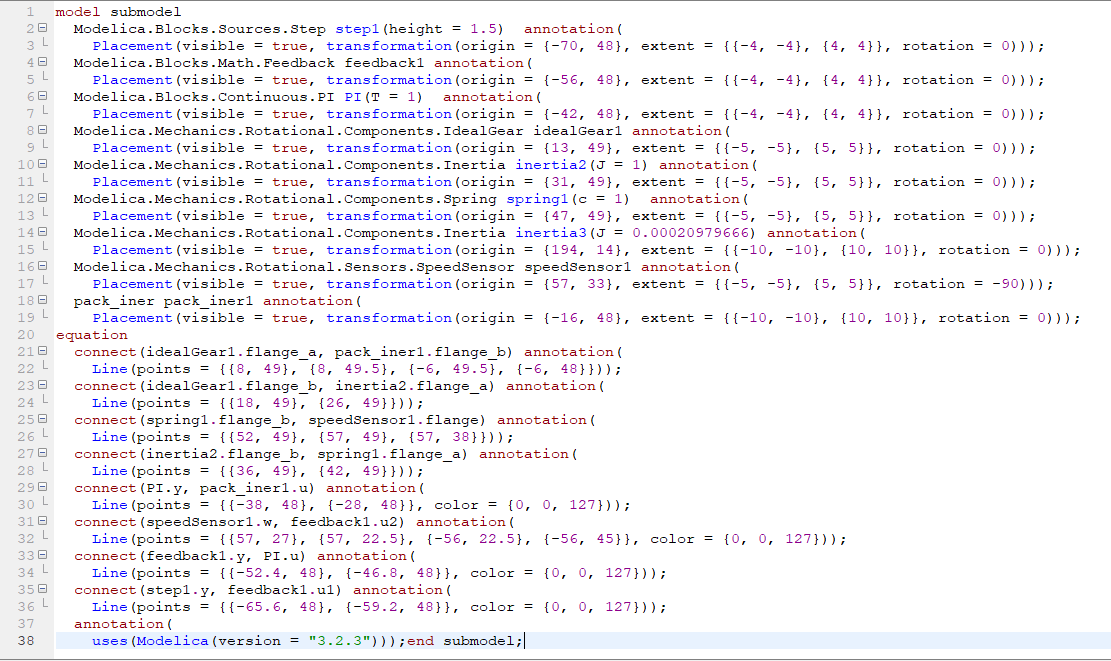
\includegraphics[width=16.5cm,height=10cm]{./Image/sub_modelica.png}
% 	\caption{図\ref{fig:submodel}のModelicaコード}
% 	\label{fig:sub_modelica}
%   \end{figure}
% 3章へ
%   \subsection{モデル作成時の制約}\label{sub:seiyaku}
%   \ref{sub:tanntai}章、\ref{sub:submodel}章で説明したモデルを作成する際は、以下の制約を満たしていなければならない。
% \subsubsection{電圧値は一定}
% 今回試作するモータ特性表自動生成ツールでは、電圧値が一定の場合に得られる特性\cite{電圧一定}も示すため、入力である電圧値は一定でなければならない。
% \subsubsection{0秒からモータを動かす}
% 今回試作するモータ特性表自動生成ツールの仕様上、モータに対して0秒から入力を与え、モータを動かすようにしなければならない。
\section{モータ特性表}\label{mortoku}
モータ特性表とは、モータを選定する際に、参考にする資料である\cite{仕様の見方}。例えば、図\ref{fig:rei_mortoku}に、示すモータ特性表の例を示す\cite{特性表4}。一般的に決まった形式はなく、企業によって掲載する要素は異なるため、
10社のブラシ付きDCモータのモータ特性表\cite{特性表1,特性表2,特性表3,特性表4,特性表5,特性表6,特性表7,特性表8,特性表9,特性表10}に含まれる要素を集計した。集計結果を、表\ref{tab:syuukei}に示す。
表\ref{tab:syuukei}で示した12個の値と4種類のグラフを、今回自動生成するモータ特性表の要素とする。
% 「無負荷電流」、「無負荷回転数」、「起動トルク」を除く理由は、\ref{sub:mortortoku}節にて述べる。
% \scalebox{0.8}{
	\begin{figure}[t]
		\centering
		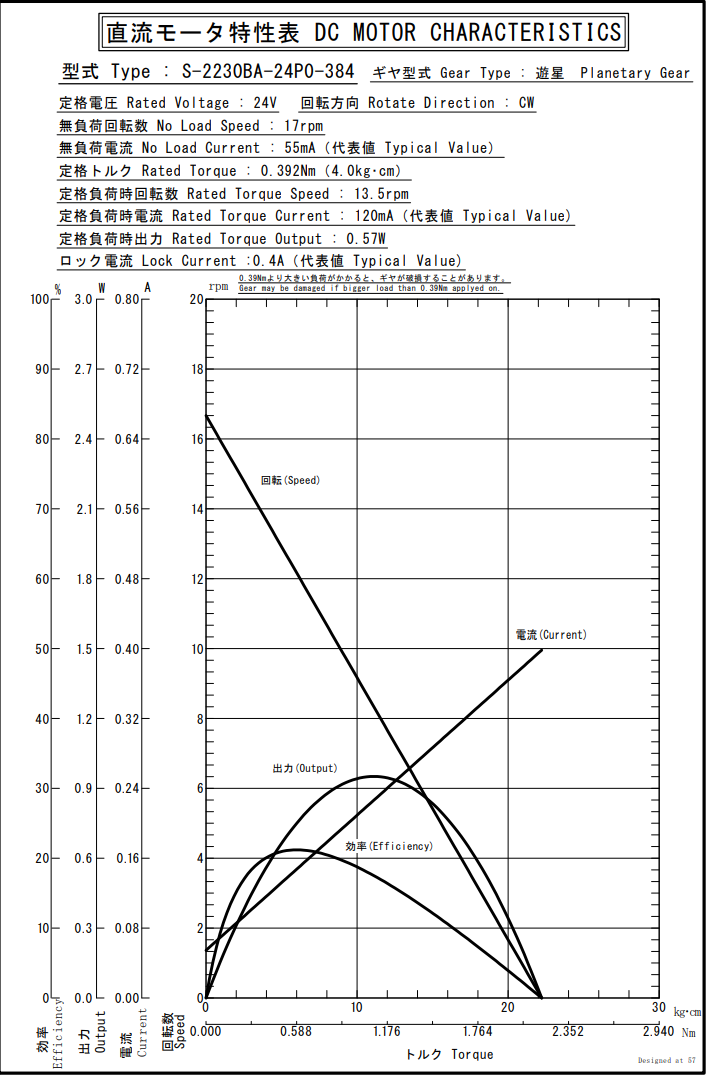
\includegraphics[width=10cm]{./Image/rei_mortoku.png}
		\caption{モータ特性表の例}
		\label{fig:rei_mortoku}
	  \end{figure} 

\begin{table}[t]
	\centering
	\caption{モータ特性表の要素の集計結果}
	\begin{tabular}{|c|c||c|c|} \hline
		要素名 & 出現回数 & 要素名 & 出現回数 \\ \hline\hline
		定格トルク & 10 & 定格出力 & 5 \\ \hline
		定格電流 & 9 & 「トルク $\times$ 効率」グラフ & 5 \\ \hline
		定格回転数 & 9 & 「トルク $\times$ 出力」グラフ & 5 \\ \hline
		無負荷電流 & 8 & 停動トルク & 4 \\ \hline
		無負荷回転数 & 8  & 始動電流 & 3 \\ \hline
		「トルク $\times$ 電流」グラフ & 7 &  最大回転数 & 2 \\ \hline
		「トルク $\times$ 回転数」グラフ & 7 & 始動トルク & 2\\ \hline
		定格電圧 & 5 & 最大効率 & 1 \\ \hline
		
		
	% \begin{tabular}{|c|c||c|c||c|c||c|c|} \hline
	%   要素名 & 出現回数 &  要素名 & 出現回数 &  要素名 & 出現回数 &  要素名 & 出現回数\\\hline\hline
	%   定格電流 & 9 &  効率 & 6 & 回転数 & 3 & 容量 & 1 \\ \hline
	%   電圧 & 8 &  枠番 & 4 & 極数 & 2 & 特記事項 & 1 \\ \hline
	%   出力 & 7 &電流 & 4 &  回転方向 & 2 & IEコード & 1 \\ \hline
	%   始動トルク & 7 & 停動トルク & 4 & 無負荷回転数 & 2 & 定格電圧 & 1 \\ \hline
	%   始動電流 & 7 & 力率 & 4 &    無負荷電流 & 2 & 停動電流 & 1  \\ \hline
	%   定格回転数 & 7 & 最大トルク & 4 &  定格出力 & 2 &ブラシ & 1  \\ \hline
	%   周波数 & 6 & 定格トルク & 3 &  慣性モーメント & 1 & ノイズ素子 & 1 \\ \hline
	\end{tabular}
	 \label{tab:syuukei}
  \end{table}
  % }
% \begin{figure}[t]
% 	\centering
% 	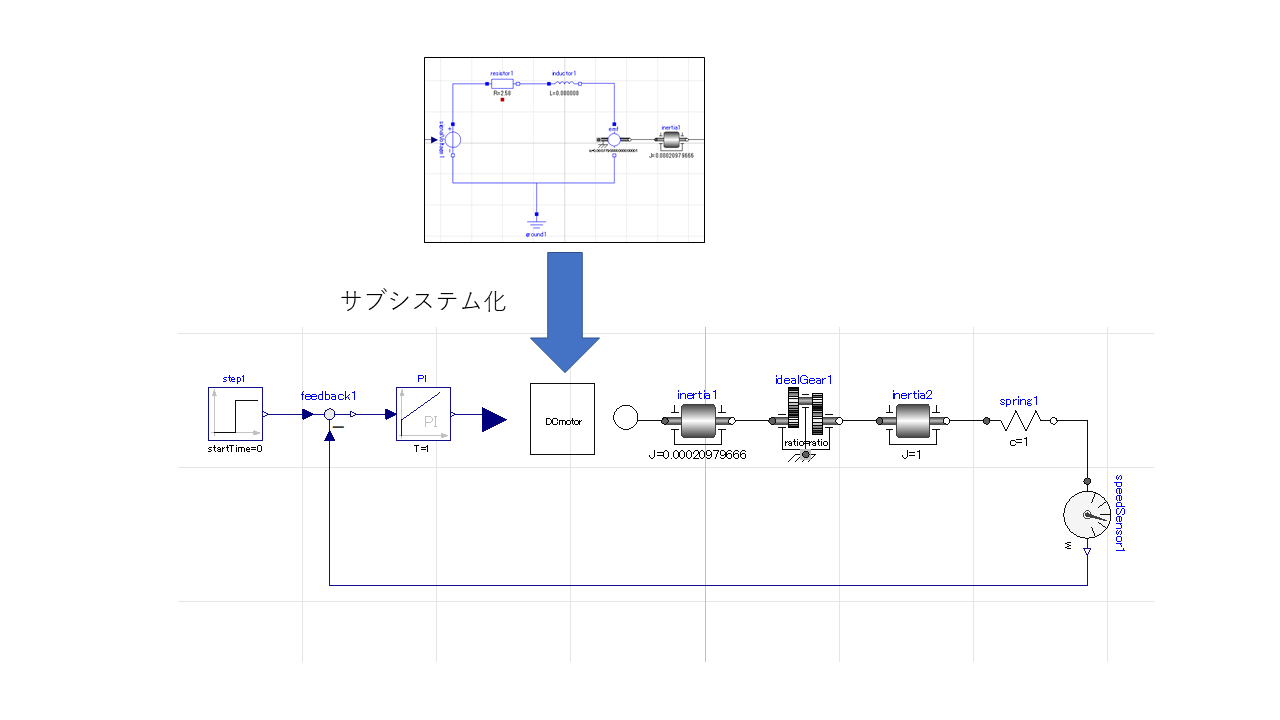
\includegraphics[width=16.5cm,height=10cm]{./Image/submodel_pack.png}
% 	\caption{モータ特性表の集計結果}
% 	\label{fig:syuukei}
%   \end{figure}

以下に、自動生成するモータ特性表の構成を示す。
\begin{itemize}
	\item モータ特性表
	\begin{itemize}
		\item 特性表
% 		\begin{itemize}
% 			\item 電圧 V
% 			\item 始動電流 mA
% 			\item 停動トルク $mN \cdot m$
% 			\item 最大効率 \%
% 			\item 定格トルク $mN \cdot m$
% 			\item 定格回転数 rpm
% 			\item 定格電流 mA
% 			\item 定格出力 W
% 			\item 最大回転数 rpm 
% 		\end{itemize}
		\item 特性グラフ
% 		\begin{itemize}
% 			\item トルク $mN \cdot m$ $\times$ 電流 mA
% 			\item トルク $mN \cdot m$ $\times$ 回転数 rpm
% 			\item トルク $mN \cdot m$ $\times$ 効率 \%
% 			\item トルク $mN \cdot m$ $\times$ 出力 W
% 		\end{itemize}
	\end{itemize}
\end{itemize}
以下で、本研究で対象とするモータ特性表の、特性表と特性グラフの内容について述べる。
\subsection{特性表}\label{sub:tokuseihyou}
特性表とは、以下の12個の値で構成する。
% \begin{itemize}
% 	\item 電圧 V
% 	\item 始動電流 mA
% 	\item 停動トルク $mN \cdot m$
% 	\item 最大効率 \%
% 	\item 定格トルク $mN \cdot m$ 
% 	\item 定格回転数 rpm
% 	\item 定格電流 mA
% 	\item 定格出力 W
% 	\item 最大回転数 rpm 
% \end{itemize}
% 以下に各要素が表す内容について述べる。
\subsubsection{定格電圧(Rated Voltage)}\label{sub:sub:dennatu}
% \subsection{電圧}\label{sub:dennatu}
定格電圧とは、モータが回転する電圧の基準値を表す。本研究では、シミュレーション時に回路に印加した電圧値を定格電圧とする。

単位は、$\mathrm{V}$である。
\subsubsection{始動電流(Starting Current)}\label{sub:sub:sidouden}
% \subsection{始動電流}\label{sub:sidouden}
始動電流とは、モータを始動する際、回路に流れる電流の最大値を表す。

単位は、$\mathrm{mA}$である。
% https://www.tsugawa.co.jp/glossary/ 

\subsubsection{無負荷電流(No-Load Current)}
無負荷電流とは、モータに負荷がかかっていないときの電流値を表す。

単位は、$\mathrm{mA}$である。

\subsubsection{無負荷回転数(No-Load Speed)}
無負荷回転数とは、モータに負荷がかかっていないときの回転数を表す。

単位は、$\mathrm{rpm}$である。

\subsubsection{始動トルク(Starting Torque)}
始動トルクとは、モータが始動する際に発生するトルクの値を表す。

単位は、$\mathrm{mN \cdot m}$である。


\subsubsection{停動トルク(Stalling Torque)}\label{sub:sub:teidoutoruku}
% \subsection{停動トルク}\label{sub:teidoutoruku}
% 停動トルクとは、モータが出しうる最大トルクで、このトルク以上の負荷がかかれば、モータが停止する値を表す。
停動トルクとは、モータが停止する負荷トルクの値を表す。負荷トルクとは、モータの回転を停止させようとする力のことである。

単位は、$\mathrm{mN \cdot m}$である。
% https://www.orientalmotor.co.jp/tech/glossary/ta11/
\subsubsection{最大効率(Maximum Efficiency)}\label{sub:sub:saidaikouritu}
% \subsection{最大効率}\label{sub:saidaikouritu}
最大効率とは、効率の最大値を表す値である。効率とは、モータに与える入力エネルギーとモータを回転させるために要した機械エネルギーの比を百分率[\%]で表した値である。入力エネルギーは電流と電圧の積で計算でき、出力エネルギーはモータの回転に加わるトルクと角速度で計算できる。

単位は、$\mathrm{\%}$である。
% https://www.jp-igarashi.com/product/product_motors/curve.html
\subsubsection{定格トルク(Rated Torque)}\label{sub:sub:teikakutoruku}
% \subsection{定格トルク}\label{sub:teikakutoruku}
定格トルクとは、最大効率時のトルク値を表す。

単位は、$\mathrm{mN \cdot m}$である。
% http://www.sagamimicro.co.jp/product/aboutusage.html
\subsubsection{定格回転数(Rated Speed)}\label{sub:sub:teikakukaiten}
% \subsection{定格回転数}\label{sub:teikakukaiten}
定格回転数とは、最大効率時のモータの回転数の値を表す。

単位は、$\mathrm{rpm}$である。

% https://mathwords.net/kaitensu
\subsubsection{定格電流(Rated Current)}\label{sub:sub:teikakuden}
% \subsection{定格電流}\label{sub:teikakuden}
定格電流とは、最大効率時の電流値を表す。

単位は、$\mathrm{mA}$である。
% http://fa-faq.mitsubishielectric.co.jp/faq/show/18504?category_id=1937&site_domain=default
\subsubsection{定格出力(Rated Power)}\label{sub:sub:teikakusyutu}
% \subsection{定格出力}\label{sub:teikakusyutu}
定格出力とは、最大効率時の出力値を表す。

単位は、$\mathrm{W}$である。
% \ref{sub:sub:teikakukaiten}章で求めた定格回転数と\ref{sub:sub:teidoutoruku}章で求めた定格トルクを
% http://www.nidec-servo.com/jp/digital/pdf/A_technique.pdf
\subsubsection{最大回転数(Maximum Speed)}\label{sub:sub:saidaikai}
% \subsection{最大回転数}\label{sub:saidaikai}
最大回転数とは、回転数の値の中で最大値を表す。

単位は、$\mathrm{rpm}$である。
\subsection{特性グラフ}\label{sub:tokuseigurahu}
特性グラフは、以下の4つのグラフで構成する。
% \begin{itemize}
% 	\item トルク $mN \cdot m$ $\times$ 電流 mA
% 	\item トルク $mN \cdot m$ $\times$ 回転数 rpm
% 	\item トルク $mN \cdot m$ $\times$ 効率 \%
% 	\item トルク $mN \cdot m$ $\times$ 出力 W
% \end{itemize}
% 以下に各グラフについて述べる。
\subsubsection{「トルク $\times$ 電流」グラフ}\label{sub:sub:torden}
「トルク $\times$ 電流」グラフとは、横軸が「トルク $(\mathrm{mN \cdot m})$」、縦軸が「電流 $(\mathrm{mA})$」のグラフである。

このグラフでは、トルクに対する電流の変化量を表す。
\subsubsection{「トルク $\times$ 回転数」グラフ}\label{sub:sub:torkaiten}
「トルク $\times$ 回転数」グラフとは、横軸が「トルク $(\mathrm{mN \cdot m})$」、縦軸が「回転数 $(\mathrm{rpm})$」のグラフである。

このグラフでは、トルクに対する回転数の変化量を表す。
\subsubsection{「トルク $\times$ 効率」グラフ}\label{sub:sub:torkouritu}
「トルク $\times$ 効率」グラフとは、横軸が「トルク $(\mathrm{mN \cdot m})$」、縦軸が「効率 $(\mathrm{\%})$」のグラフである。

このグラフでは、トルクに対する効率の変化量を表す。
\subsubsection{「トルク $\times$ 出力」グラフ}\label{sub:sub:torsyutu}
「トルク $\times$ 出力」グラフとは、横軸が「トルク $(\mathrm{mN \cdot m})$」、縦軸が「出力 $(\mathrm{W})$」のグラフである。

このグラフでは、トルクに対する出力の変化量を表す。
\section{Python}\label{python}
Pythonは、1991年にオランダ人のグイド・ヴァンロッサムによって開発され、オープンソースで運営されている動的プログラミング言語である\cite{pythonoya}。
Pythonの用途は様々で、組込み開発や、Webアプリケーション、デスクトップアプリケーション、さらには人工知能開発、ビッグデータ解析などと多岐に渡る\cite{pythonsamu}。
Pythonのプログラミング言語としての主な特徴は、少ないコードで簡潔にプログラムを書けること、専門的なライブラリが豊富にあることが挙げられる。

% pythonのバージョンは3.8.0
今回試作するモータ特性表自動生成ツールの開発言語には、Pythonを用いる。
また、使用するPythonのライブラリを、表\ref{tab:libr}に示す。
\begin{table}[t]
	\centering
	\caption{使用するPythonのライブラリ}
	\begin{tabular}{|c|c|} \hline
	  ライブラリ & 役割\\ \hline \hline
	  csv & csvファイルの操作 \\ \hline
	  math &  数学関数の使用\\ \hline
	  matplotlib & グラフ描画\\ \hline
	  numpy &  配列の計算\\ \hline
	  decimal &  指数表記の計算\\ \hline
	  reportlab & PDFファイル作成 \\ \hline
	  PIL &  画像処理\\ \hline
	  pdf2image &  PDFファイルの画像化\\ \hline
	  sys & スクリプトの起動パラメータの取得\\ \hline
	  os &  不要なファイルの削除\\ \hline
	\end{tabular}
	\label{tab:libr}
  \end{table}

% \begin{itemize}
% 	\item csv
% 	\item math
% 	\item matplotlib
% 	\item numpy
% 	\item decimal
% 	\item reportlab
% 	\item PIL
% 	\item pdf2image
% 	\item sys
% 	\item os
% \end{itemize}
% avaは、1990年代前半にSun MicrosystemsでJames Arthur Gosling、Wiliam Nelson Joyなどの人々が開発したプログラミング言語およびプラットフォームである。
% Javaはクラスベースのオブジェクト指向プログラミング言語である。
% Javaのプログラムは複数のクラスから構成され、クラス定義からそのクラスのインスタンスであるオブジェクトを何個でも作ることができる%\cite{プログラミング言語Java}。

% 1つのjavaファイルには複数のクラスを記述できる。
% 各クラスにはメンバが存在し、メンバの主な種類はフィールドとメソッドである。
% フィールドは、クラス自身あるいはそのクラスのオブジェクトのどちらかに属しているデータ変数である。
% メソッドは、クラスの状態を操作するためにフィールドに対して実行可能な処理を行う振舞いである。

% 今回実装は、で開発する。